\begin{center}
\vspace*{5.5cm}
\huge{\textbf{\textcolor[HTML]{D32F2F}{Appendix}}}
\end{center}
\newpage 

\appendix
\section{\textcolor[HTML]{D32F2F}{Spørreundersøkelse – Resultater}} \label{App:AppendixA}

Gruppen fikk inn 51 svar på spørreundersøkelsen som ble sendt ut i forbindelse med prosjektet. Resultatene følger.

\begin{figure}[H]
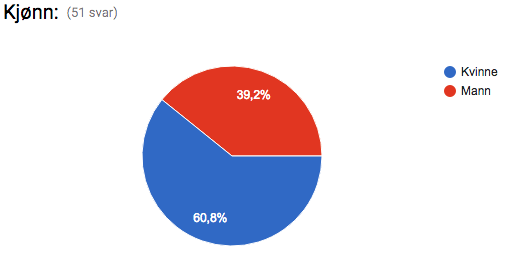
\includegraphics[scale=0.6]{images/sporreundersokelse/kjonn}
\centering %centering the image
\caption{Kjønn}
\label{fig:kjonn}
\end{figure}

\begin{figure}[H]
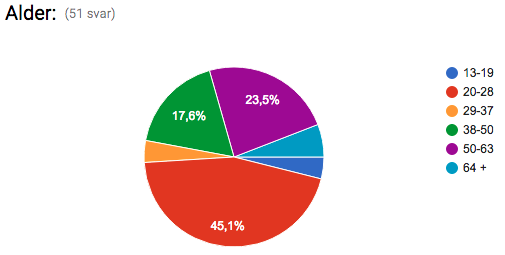
\includegraphics[scale=0.6]{images/sporreundersokelse/alder}
\centering %centering the image
\caption{Alder}
\label{fig:alder}
\end{figure}

\begin{figure}[H]
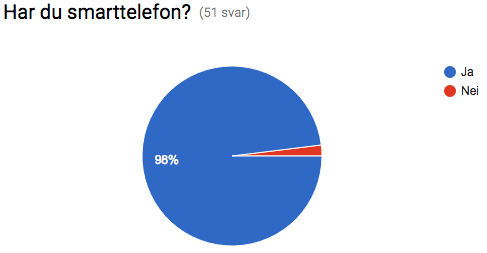
\includegraphics[scale=0.6]{images/sporreundersokelse/smarttelefon}
\centering %centering the image
\caption{Eier smarttelefon}
\label{fig:smarttelefon}
\end{figure}

\begin{figure}[H]
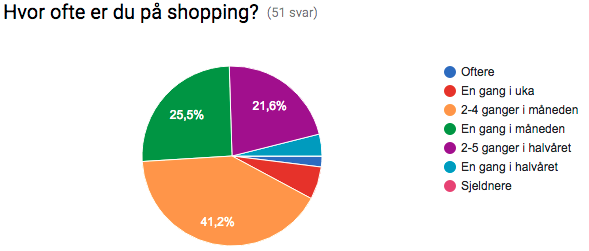
\includegraphics[scale=0.6]{images/sporreundersokelse/shopping}
\centering %centering the image
\caption{Shoppingfrekvens}
\label{fig:shopping}
\end{figure}

\begin{figure}[H]
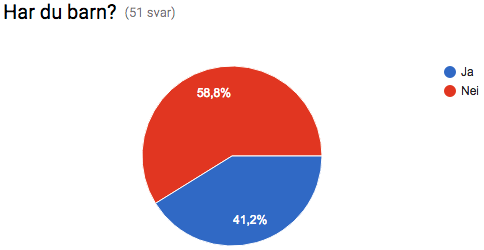
\includegraphics[scale=0.6]{images/sporreundersokelse/barn}
\centering %centering the image
\caption{Barn}
\label{fig:barn}
\end{figure}

\begin{figure}[H]
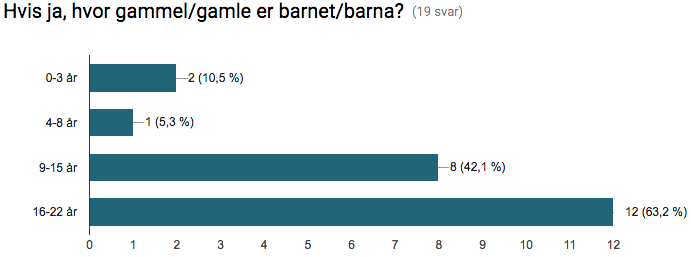
\includegraphics[scale=0.6]{images/sporreundersokelse/alderbarn}
\centering %centering the image
\caption{Alder på barn}
\label{fig:alderbarn}
\end{figure}

\noindent \large{\textbf{Hvis ja, hvordan opplever du handleturen med barna?}}
\begin{itemize}
    \item Trivelig
    \item Trivelig
    \item Stressende
    \item OK
    \item Hyggelig. Får gode råd og tips av nesten voksen datter.
    \item Tragisk, de ber alltid om noe
    \item Helt OK
    \item Bra
    \item Litt stressende :)
    \item Barna er voksne…
    \item Koselig
    \item Er så voksne at det bare er hyggelig
    \item Hyggelig, får råd og hjelp
\end{itemize}

\begin{figure}[H]
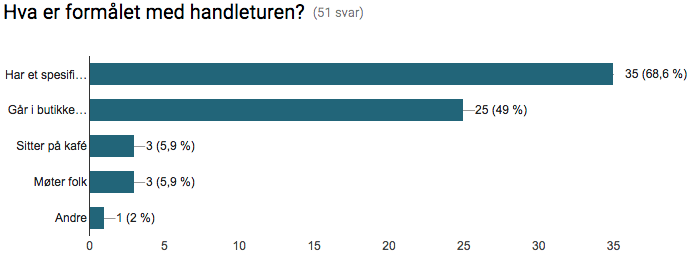
\includegraphics[scale=0.6]{images/sporreundersokelse/formal}
\centering %centering the image
\caption{Formål med handletur}
\label{fig:formal}
\end{figure}

\begin{figure}[H]
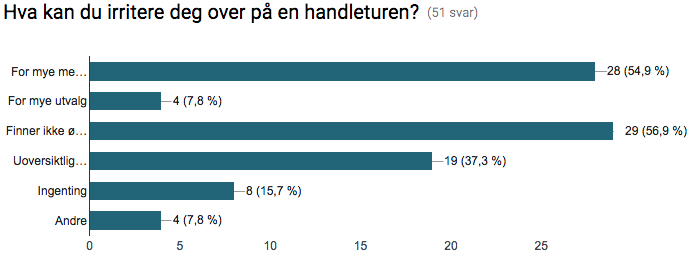
\includegraphics[scale=0.6]{images/sporreundersokelse/irritasjonsmoment}
\centering %centering the image
\caption{Irritasjonsmoment}
\label{fig:irritasjonsmoment}
\end{figure}

\begin{figure}[H]
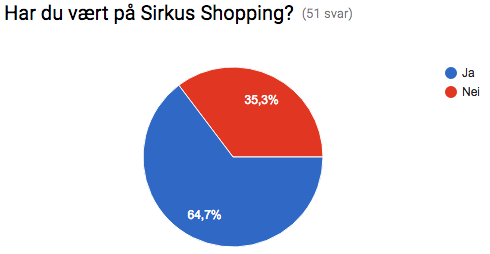
\includegraphics[scale=0.6]{images/sporreundersokelse/besokt}
\centering %centering the image
\caption{Besøkt Sirkus shopping}
\label{fig:besokt}
\end{figure}

\noindent \large{\textbf{Hvis ja, hvordan opplever du handleturen på Sirkus shopping?}}
\begin{itemize}
    \item Ok
    \item Ok
    \item Bra
    \item Bra
    \item Helt OK
    \item Helt ok
    \item Rotete
    \item Rotete
    \item Fint
    \item Fint
    \item Hva er Sirkus Shopping?
    \item Veldig bra
    \item Fin
    \item Rolig affære, finner sjelden noe
    \item Husker ikke
    \item Rolig
    \item Veldig fint kjøpesenter, lett å finne fram
    \item Bra!
    \item Litt rar planløsning, men var ikke et så masete sted
    \item Stort senter, vanskelig å få god oversikt. Behagelig pga mindre folk.
    \item Liker sirkus. Åpent og god oversikt, pleier ikke være så mye folk
    \item OK
    \item Litt uoversiktlig
    \item Den var bra! et lett og finne fram og ryddig
    \item Bra
    \item Tilfredsstillende
    \item Veldig stort og uoversiktlig
    \item God opplevelse, nyttige sofaer dårlig for menn, utvalg
    \item Helt greit. God plass, enkel parkering, kan få vasket bilen mens du handler, litt “andre” butikker
    \item Husker ikke. Lenge siden jeg var der
    \item Helt greit. Grei parkering, får vasket bilen mens du handler. Litt annerledes butikker.
\end{itemize}

\noindent \large{\textbf{Har du brukt apper for å forbedre shoppingen tidligere, evt. hvilke?}}
\begin{itemize}
    \item Nei
    \item Ja, mattilbud
    \item Nei, teknologi er ikke noe for meg
    \item Ingen
    \item Prisjakt.no, finn, google-søk om varene
    \item ikke en app laget for kjøpesenter, men bestilt varer på app tidligere og fått de levert på døra
    \item Zalando
\end{itemize}

\begin{figure}[H]
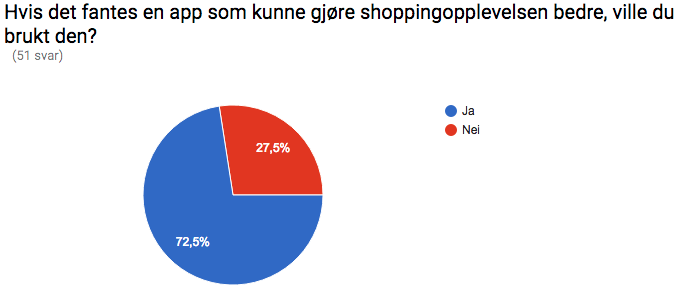
\includegraphics[scale=0.6]{images/sporreundersokelse/brukeapp}
\centering %centering the image
\caption{Vil bruke app}
\label{fig:brukeapp}
\end{figure}

\noindent \large{\textbf{Hvis nei, hvorfor?}}
\begin{itemize}
    \item For mange apper
    \item For mange apper
    \item Fordi jeg vil ikke i butikken i det hele tatt
    \item Shopper lite
    \item Hva er en app?
    \item Bestiller alt online
    \item Jeg shopper så og si aldri
    \item Synes det er lite vits, da jeg uansett er på shopping for å titte og se meg rundt
    \item Jeg kan bruke den hvis det er noe spesifikt jeg trenger som jeg vil se etter på tilbud. Ellers så liker jeg å gå rundt i butikker og prøve ulike varianter av et produkt før jeg gjør et kjøp
    \item Er ikke så ofte på shopping at jeg føler jeg har behov for en shoppingapp. Tar bare plass på telefonen. Men kommer selvfølgelig an på hva en slik app inneholder også.
    \item Enda mer å styre med bare
    \item Ser ikke behovet
    \item Ikke interessert
\end{itemize}

\noindent \large{\textbf{Har du forslag til funksjoner en shopping-app kan inneholde??}}
\begin{itemize}
    \item Nei
    \item Lagerbeholdning, pris, tester
    \item Viser hva er i butikken - størrelser utvalg osv. for å unngå bomturer
    \item Litt usikker
    \item Oversikt over butikker
    \item Hvor man finner nærmeste toalett, at man kan legge inn at man f.eks.. ønsker å kjøpe hvit skjerf så kommer forslag til butikker som har dette skjerfet
    \item Oversikt over nåværende tilbud
    \item nei dessverre
    \item Rabatt koder
    \item Alle butikker, priser og salg hos hver enkelt kjøpesenter
    \item Prissammenligning
    \item Lageroversikt
    \item Tilbud fra butikkene
    \item Salstilbud, oversikt over butikker
    \item Oversikt over hva som faktisk finnes i de ulike butikkene, ikke bare online
    \item Oversikt over hvor jeg kan finne ønsket produkt
    \item Rabattkort/kuponger?
    \item App er ut, Finn på noe nytt
    \item rabatter, kart over senter, en knapp som får små barn til å slutte å gråte
    \item Oversikt over rabatter og tilbud, info om hvor crowded en butikk er (så jeg kan unngå butikken), hvem som er på jobb i butikken jeg vil besøke (hvis det er spesielle selgere man har opparbeidet seg relasjon med)
    \item Konkurranser og ekstra tilbud forbeholdt brukere av appen (da ville jeg ha lastet den ned, selv om jeg ikke er på shopping så ofte). Kart med oversikt over de ulike butikkene kan også være nyttig.
    \item Oversikt over tilgjengelige produkter og pris
    \item Strekkodescanner som gir deg nyttig info om produktet, prissammenligning, peer reviews og promovideo
    \item Størrelser på klær sko. Nyheter.
    \item Kart over shoppingsenteret med gps som finner din posisjon. Kan også ha et side med alle tilbud på senteret.
    \item Oversikt over produkter, størrelser, hvor man finner de, pris, antall og om de evt. er på lageret om de ikke er ute i butikken. Når produktet evt kommer inn igjen om det ikke finnes p.t.
    \item Kupp
    \item Babes of the day
    \item ukestilbud/dagstilbud. hvilke butikker som er tilgjengelig og hvor de holder til/åpningstider. hvor man kan kjøpe mat og kanskje en slags for kunde-rating for andre brukere på appen så man kan ta utgangspunkt i det når man skal ha “matpause” fra shoppingen. en kommentarfelt til hver butikk hvor man kan legge en tilbakemelding etter endt shopping, og slik at andre potensielle kunder kan se om servicen er bra der osv.
    \item Nei
    \item Bilde av klærne på en som er ca samme strl
    \item Nærmeste utsalg av produktet
    \item Salgsvarer. Sesongvarer
    \item vet ikke
    \item Merker, hvilke butikker har hvilke merker
    \item Kart over kjøpesenter for å finne butikkene. Søke etter hvilken butikk som har den varen man ønsker å kjøpe
    \item Hvilke butikker som har hvilke merker
\end{itemize}

\newpage
\section{\textcolor[HTML]{D32F2F}{Observasjonsskjema for test 1}} \label{App:AppendixB}

\begin{table}[H]
    \caption{Sivilingeniør 58 år, dame}
    \label{tab:observasjon1_1}
    \centering
    \begin{tabular}{L{15em}  L{15em} L{15em}}
        \rowcolor[HTML]{D32F2F}
        \textbf{\textcolor{white}{Task}} & \textbf{\textcolor{white}{Obeservation during execution}} & \textbf{\textcolor{white}{Conversation and discussion}}\\
        \rowcolor[HTML]{E6E6E6}
        1. Du skal lage en oversikt over dine bursdagsønsker. Lista skal hete “bursdagsønsker”. & “Bra å få vite åpningstid”. Laget lista. Bra & \\
        2. Du har nå opprettet tre ulike handlelister. Naviger deg frem til en oversikt over disse. & Trykket på Mine handlelister. Bra &  \\
        \rowcolor[HTML]{E6E6E6}
        3. Legg til en genser i listen over bursdagsønsker. & Går på bursdagsønsker. Trykker på legg til i handlekurv. Tenker lenge. Kommer etterhvert på at man kan scanne klær. Velger størrelse. Legg i handlekurv & Glemmer beskjeden i begynnelsen. Savner et skjermbilde som gjør klar for scanning.\\ 
        4. Genseren du har lagt i handlelisten er i feil størrelse. Bytt størrelse. & Trykker tilbake. (Kommer da til bilde av genseren. Vet ikke om det er det som skal skje) Skifter størrelse. Trykker legg i handlekurv. & Ønsker en beskjed om hva som har skjedd.\\
        \rowcolor[HTML]{E6E6E6}
        5. Du vil ikke lenger ha genseren. Fjern genseren. & Trykker på søppelbøtta. Bra & \\
        6. Du har nå lagt til tre varer til listen og handleturen din er ferdig. Kjøp varene i handlekurven. & Trykker lagre. Går inn på bursdagsønsker igjen. “Har jo lagt det i handlekurva før?” Trykker legg til i handlekurv. Lever bestilling. Betal i kasse. & Ville ikke ha brukt systemet hvis man må vente til slutt. Kan like godt ta med varene selv.\\
        \rowcolor[HTML]{E6E6E6}
        7. Du er på oversikten over dine handlelister. Naviger deg tilbake til startsiden. & Trykker tilbake & \\
        8. Du har fylt opp handlekurven din, men ønsker ikke å kjøpe med én gang. Hva gjør du? & Trykker lagre & \\
    \end{tabular}
\end{table}

\noindent SUS result: 57,5

\begin{table}[H]
    \caption{Student 24 år, jente}
    \label{tab:observasjon1_2}
    \centering
    \begin{tabular}{L{15em}  L{15em} L{15em}}
        \rowcolor[HTML]{D32F2F}
        \textbf{\textcolor{white}{Task}} & \textbf{\textcolor{white}{Obeservation during execution}} & \textbf{\textcolor{white}{Conversation and discussion}}\\
        \rowcolor[HTML]{E6E6E6}
        1. Du skal lage en oversikt over dine bursdagsønsker. Lista skal hete “bursdagsønsker”. & Bra. & \\
        2. Du har nå opprettet tre ulike handlelister. Naviger deg frem til en oversikt over disse. & Trykker tilbake. Mine handlelister. Bra &  \\
        \rowcolor[HTML]{E6E6E6}
        3. Legg til en genser i listen over bursdagsønsker. & Går på bursdagsønsker. Trykker legg til i handlekurv. Går tilbake til hovedmeny. Bursdagsønsker. Legg til i handlekurv. Leter etter en plass for å scanne. Gir henne et hint. Scanner genseren. Trykker legg til i handleliste. & Husker ikke at man bare skal scanne. Kunne hatt en knapp i hjørnet.\\
        4. Genseren du har lagt i handlelisten er i feil størrelse. Bytt størrelse. & Sletter genseren. Scanner den på nytt og legger til en ny. & \\
        \rowcolor[HTML]{E6E6E6}
        5. Du vil ikke lenger ha genseren. Fjern genseren. & Trykker søppelbøtta & \\
        6. Du har nå lagt til tre varer til listen og handleturen din er ferdig. Kjøp varene i handlekurven. & Trykker legg i handlekurv og lever bestilling. Gikk bra. & \\
        \rowcolor[HTML]{E6E6E6}
        7. Du er på oversikten over dine handlelister. Naviger deg tilbake til startsiden. & Ok & \\
        8. Du har fylt opp handlekurven din, men ønsker ikke å kjøpe med én gang. Hva gjør du? & Går til bursdagsønsker. (Gir henne handlekurvbilde, mangler noe i mellom her). Trykker lagre. & Skjønner ikke helt forskjell på liste og kurv. Hvis du scanner og skal kjøpe, legger du i kurv. Hvis du ikke skal kjøpe den, er det noe du ønsker deg.\\
    \end{tabular}
\end{table}

\noindent SUS result: 87,5

\begin{table}[H]
    \caption{Student 22 år, gutt}
    \label{tab:observasjon1_3}
    \centering
    \begin{tabular}{L{15em}  L{15em} L{15em}}
        \rowcolor[HTML]{D32F2F}
        \textbf{\textcolor{white}{Task}} & \textbf{\textcolor{white}{Obeservation during execution}} & \textbf{\textcolor{white}{Conversation and discussion}}\\
        \rowcolor[HTML]{E6E6E6}
        1. Du skal lage en oversikt over dine bursdagsønsker. Lista skal hete “bursdagsønsker”. & Bra. & \\
        2. Du har nå opprettet tre ulike handlelister. Naviger deg frem til en oversikt over disse. & Trykker tilbake. Bra &  \\
        \rowcolor[HTML]{E6E6E6}
        3. Legg til en genser i listen over bursdagsønsker. & Trykker bursdagsønsker. Scanner med en gang. Velger størrelse. Trykker legg til i handleliste. Bra & \\
        4. Genseren du har lagt i handlelisten er i feil størrelse. Bytt størrelse. & Trykker på genseren som ligger i lista. Bytter størrelse. Trykker tilbake. Skjønte ikke helt hva han gjorde. “Er størrelsen endret nå?” & \\
        \rowcolor[HTML]{E6E6E6}
        5. Du vil ikke lenger ha genseren. Fjern genseren. & Trykker på søppelbøtta. Bra & \\
        6. Du har nå lagt til tre varer til listen og handleturen din er ferdig. Kjøp varene i handlekurven. & Trykker legg til i handlekurv. Lever bestilling. Betal med vipps. Bra & \\
        \rowcolor[HTML]{E6E6E6}
        7. Du er på oversikten over dine handlelister. Naviger deg tilbake til startsiden. & Trykker tilbake & \\
        8. Du har fylt opp handlekurven din, men ønsker ikke å kjøpe med én gang. Hva gjør du? & Usikker på hva som skal gjøres. Leter etter handlekurva. Går inn på bursdagsønsker og legg til i handlekurv. & Handleliste og kurv ser så like ut, vanskelig å se forskjell. Foreslår å bare ha kurver og ikke lister..\\
    \end{tabular}
\end{table}

\noindent SUS result: 77,5

\begin{table}[H]
    \caption{Student 23 år, gutt}
    \label{tab:observasjon1_4}
    \centering
    \begin{tabular}{L{15em}  L{15em} L{15em}}
        \rowcolor[HTML]{D32F2F}
        \textbf{\textcolor{white}{Task}} & \textbf{\textcolor{white}{Obeservation during execution}} & \textbf{\textcolor{white}{Conversation and discussion}}\\
        \rowcolor[HTML]{E6E6E6}
        1. Du skal lage en oversikt over dine bursdagsønsker. Lista skal hete “bursdagsønsker”. & Logger inn. Ny handleliste. Alt bra. & \\
        2. Du har nå opprettet tre ulike handlelister. Naviger deg frem til en oversikt over disse. & Trykker tilbake. Trykker mine handlelister. Bra &  \\
        \rowcolor[HTML]{E6E6E6}
        3. Legg til en genser i listen over bursdagsønsker. & Trykker på bursdagsønsker. Trykker Legg til i handlekurv. Går tilbake. Blir forvirret. Bare prøver å scanne. Trykker legg til i handleliste. & Gir ikke mening å ha handlelister liggende. Heller ha ønskelister.\\
        4. Genseren du har lagt i handlelisten er i feil størrelse. Bytt størrelse. & Trykker på genseren i lista. Endrer størrelse. Trykker tilbake og tenker da at det blir oppdatert. Usikker på om det blir lagret. Ville hatt en melding. & \\
        \rowcolor[HTML]{E6E6E6}
        5. Du vil ikke lenger ha genseren. Fjern genseren. & Bra & \\
        6. Du har nå lagt til tre varer til listen og handleturen din er ferdig. Kjøp varene i handlekurven. & Er i bursdagsønskelista. Trykker tilbake helt til startsiden. Går inn igjen i handlelista. Prøver å trykke legg til i handlekurv, men skjønner ikke hvorfor. Tror ikke han skjønner at det i lista ikke er lagt til i handlekurva. Lever bestilling. Betal med vipps. & Forvirret mellom liste og kurv.\\
        \rowcolor[HTML]{E6E6E6}
        7. Du er på oversikten over dine handlelister. Naviger deg tilbake til startsiden. & Trykker tilbake & \\
        8. Du har fylt opp handlekurven din, men ønsker ikke å kjøpe med én gang. Hva gjør du? & Er i handlekurv. Trykker lagre. & \\
    \end{tabular}
\end{table}

\noindent SUS result: 77,5

\begin{table}[H]
    \caption{Student 22 år, jente}
    \label{tab:observasjon1_5}
    \centering
    \begin{tabular}{L{15em}  L{15em} L{15em}}
        \rowcolor[HTML]{D32F2F}
        \textbf{\textcolor{white}{Task}} & \textbf{\textcolor{white}{Obeservation during execution}} & \textbf{\textcolor{white}{Conversation and discussion}}\\
        \rowcolor[HTML]{E6E6E6}
        1. Du skal lage en oversikt over dine bursdagsønsker. Lista skal hete “bursdagsønsker”. & Logger inn. Got it. Ny handleliste. Bra & \\
        2. Du har nå opprettet tre ulike handlelister. Naviger deg frem til en oversikt over disse. & Trykker tilbake. Mine handlelister. Bra. &  \\
        \rowcolor[HTML]{E6E6E6}
        3. Legg til en genser i listen over bursdagsønsker. & Trykker på bursdagsønsker. Tenker. Trykker legg til i handlekurv. Leter etter en knapp for å scanne. Går fram og tilbake. Gir et hint. Da scanner hun. Trykker legg til i handleliste. Bursdagsønsker. & Vanskelig å skjønne når man skal scanne. Glemmer den første beskjeden, bare trykker OK.\\
        4. Genseren du har lagt i handlelisten er i feil størrelse. Bytt størrelse. & Spør om hun må trykke på genseren eller fjerne den. La til en ny genser så hun fikk to. & \\
        \rowcolor[HTML]{E6E6E6}
        5. Du vil ikke lenger ha genseren. Fjern genseren. & Trykker søppelbøtta & \\
        6. Du har nå lagt til tre varer til listen og handleturen din er ferdig. Kjøp varene i handlekurven. & Trykker legg i handlekurv. Lever bestilling. Betal i kasse. Bra &\\
        \rowcolor[HTML]{E6E6E6}
        7. Du er på oversikten over dine handlelister. Naviger deg tilbake til startsiden. & Ok & \\
        8. Du har fylt opp handlekurven din, men ønsker ikke å kjøpe med én gang. Hva gjør du? & Trykker tilbake. & \\
    \end{tabular}
\end{table}

\noindent SUS result: 95

\newpage
\section{\textcolor[HTML]{D32F2F}{Observasjonsskjema for test 2}} \label{App:AppendixC}

\begin{table}[H]
    \caption{Student 23 år, gutt}
    \label{tab:observasjon2_1}
    \centering
    \begin{tabular}{L{15em}  L{15em} L{15em}}
        \rowcolor[HTML]{D32F2F}
        \textbf{\textcolor{white}{Task}} & \textbf{\textcolor{white}{Obeservation during execution}} & \textbf{\textcolor{white}{Conversation and discussion}}\\
        \rowcolor[HTML]{E6E6E6}
        1. Du skal lage en oversikt over dine bursdagsønsker. Lista skal hete “bursdagsønsker”. & Velger å logge inn med rundingene          & Synes rundingene passet best\\
        2. Du har nå opprettet tre ulike handlelister. Naviger deg frem til en oversikt over disse. & Ok & \\
        \rowcolor[HTML]{E6E6E6}
        3. Legg til en genser i listen over bursdagsønsker. & Ok & \\ 
        4. Genseren du har lagt i handlelisten er i feil størrelse. Bytt størrelse. & Savner feedback på bytte av størrelse & \\
        \rowcolor[HTML]{E6E6E6}
        5. Du vil ikke lenger ha genseren. Fjern genseren. & Ok & \\
        6. Du har nå lagt til tre varer til listen og handleturen din er ferdig. Kjøp varene i handlekurven. & Drar alle varer fra ønskelista til ikonene & Ville heller hatt en “alle” knapp som sender alle varer til handlekurven. \\
        \rowcolor[HTML]{E6E6E6}
        7. Du er på oversikten over dine handlelister. Naviger deg tilbake til startsiden. & Ok & \\
        8. Du har fylt opp handlekurven din, men ønsker ikke å kjøpe med én gang. Hva gjør du? & Ok & \\
        \rowcolor[HTML]{E6E6E6}
        9. Del genseren med en venn & Ok & \\
    \end{tabular}
\end{table}

\begin{table}[H]
    \caption{Student 22 år, gutt}
    \label{tab:observasjon2_2}
    \centering
    \begin{tabular}{L{15em}  L{15em} L{15em}}
        \rowcolor[HTML]{D32F2F}
        \textbf{\textcolor{white}{Task}} & \textbf{\textcolor{white}{Obeservation during execution}} & \textbf{\textcolor{white}{Conversation and discussion}}\\
        \rowcolor[HTML]{E6E6E6}
        1. Du skal lage en oversikt over dine bursdagsønsker. Lista skal hete “bursdagsønsker”. & Logger på med firkantede knapper og Facebook & Synes firkantene passet best\\
        2. Du har nå opprettet tre ulike handlelister. Naviger deg frem til en oversikt over disse. & Trykker ikke på hjerte-ikonet & Vanskelig å forstå hurtigknappen med en gang \\
        \rowcolor[HTML]{E6E6E6}
        3. Legg til en genser i listen over bursdagsønsker. & Ok & \\ 
        4. Genseren du har lagt i handlelisten er i feil størrelse. Bytt størrelse. & Ok & \\
        \rowcolor[HTML]{E6E6E6}
        5. Du vil ikke lenger ha genseren. Fjern genseren. & Ok & \\
        6. Du har nå lagt til tre varer til listen og handleturen din er ferdig. Kjøp varene i handlekurven. & Dro ikke varene i knappen “legg til i handlekurv” men trykket bare på knappen & \\
        \rowcolor[HTML]{E6E6E6}
        7. Du er på oversikten over dine handlelister. Naviger deg tilbake til startsiden. & Ok & \\
        8. Du har fylt opp handlekurven din, men ønsker ikke å kjøpe med én gang. Hva gjør du? & Vil ikke gjøre noe. & Nødvendig med tilbake-knapp?\\
        \rowcolor[HTML]{E6E6E6}
        9. Del genseren med en venn & Ok & \\
    \end{tabular}
\end{table}

\begin{table}[H]
    \caption{Student 22 år, jente}
    \label{tab:observasjon2_3}
    \centering
    \begin{tabular}{L{15em}  L{15em} L{15em}}
        \rowcolor[HTML]{D32F2F}
        \textbf{\textcolor{white}{Task}} & \textbf{\textcolor{white}{Obeservation during execution}} & \textbf{\textcolor{white}{Conversation and discussion}}\\
        \rowcolor[HTML]{E6E6E6}
        1. Du skal lage en oversikt over dine bursdagsønsker. Lista skal hete “bursdagsønsker”. & Velger å logge inn med firkantene & Synes firkantene passet best\\
        2. Du har nå opprettet tre ulike handlelister. Naviger deg frem til en oversikt over disse. & Brukte ikke hjerte-ikonet & Trenger man dette eller er det noe man vil venne seg til etterhvert? \\
        \rowcolor[HTML]{E6E6E6}
        3. Legg til en genser i listen over bursdagsønsker. & Ok & \\ 
        4. Genseren du har lagt i handlelisten er i feil størrelse. Bytt størrelse. & Hvor skal man trykke etter å ha endret størrelse & Ingen feedback\\
        \rowcolor[HTML]{E6E6E6}
        5. Du vil ikke lenger ha genseren. Fjern genseren. & Ok & \\
        6. Du har nå lagt til tre varer til listen og handleturen din er ferdig. Kjøp varene i handlekurven. & Drar alle varer fra ønskelista til ikonene & Ville heller hatt en “alle” knapp som sender alle varer til handlekurven.\\
        \rowcolor[HTML]{E6E6E6}
        7. Du er på oversikten over dine handlelister. Naviger deg tilbake til startsiden. & Ville først trykke tilbake-pilen, men la merke til hjem-knappen og ønsket å trykke der istedet & \\
        8. Du har fylt opp handlekurven din, men ønsker ikke å kjøpe med én gang. Hva gjør du? & Ok & \\
        \rowcolor[HTML]{E6E6E6}
        9. Del genseren med en venn & Forstod ikke først del-knappen & Anbefaler å ha tekst i tillegg til velkjente pilen\\
    \end{tabular}
\end{table}
